\chapter{Propuesta}\label{chapter:proposal}

%La propuesta se centra en una propuesta de metalearning sobre el espacio de busqueda y utilizar el conocimiento generado por otros usuarios

La propuesta de meta-learning implementada se centra en un análisis sobre
una descripción de problemas, definiendo como espacio de búsqueda los elementos
característicos de los mismos. Dicho análisis se realiza sobre conocimiento
previo, generado por los usuarios, el cual, en los sistemas clásicos de AutoML
es desechado, causando la pérdida de los mismos y la necesidad de un
reentrenamiento de los modelos en futuros análisis.

Por lo tanto, la propuesta hecha surge de la necesidad del reaprovechamiento
del conocimiento generado en un momento dado, el cual servirá para
procesamientos de problemas venideros, obteniendo una mejora en cuanto a costo
temporal de los procesamientos sin la necesidad de recomputar soluciones
enteras desde un principio.

%COncretar el enfoque de la propuesta, que aprovecho de los usuarios anteriores.
%Importa el problema e importa los pipeline evaluados

Dicha propuesta se basa entonces en guardar características que describan los
conjuntos de datos, igualmente se salvan las soluciones más prometedoras, las
cuales se obtuvieron de análisis previos de dichos conjuntos de datos. Estas
características servirán para representar similitud entre problemas y
relacionar las soluciones con mayor posibilidad de encajar en los mismos, de
esta forma se gana en tiempo de ejecución de una solución y se evita la
exploración de soluciones no factibles.

%Diagrama de la propuesta 

\section{Diagrama de la Propuesta}

%Explicar el diagrama, explicar el flujo

El flujo de ejecución de la propuesta consta de varios pasos, como se muestra
en la Figura \ref{fig:prop-flow}.

\begin{figure}[H]
    \centering
    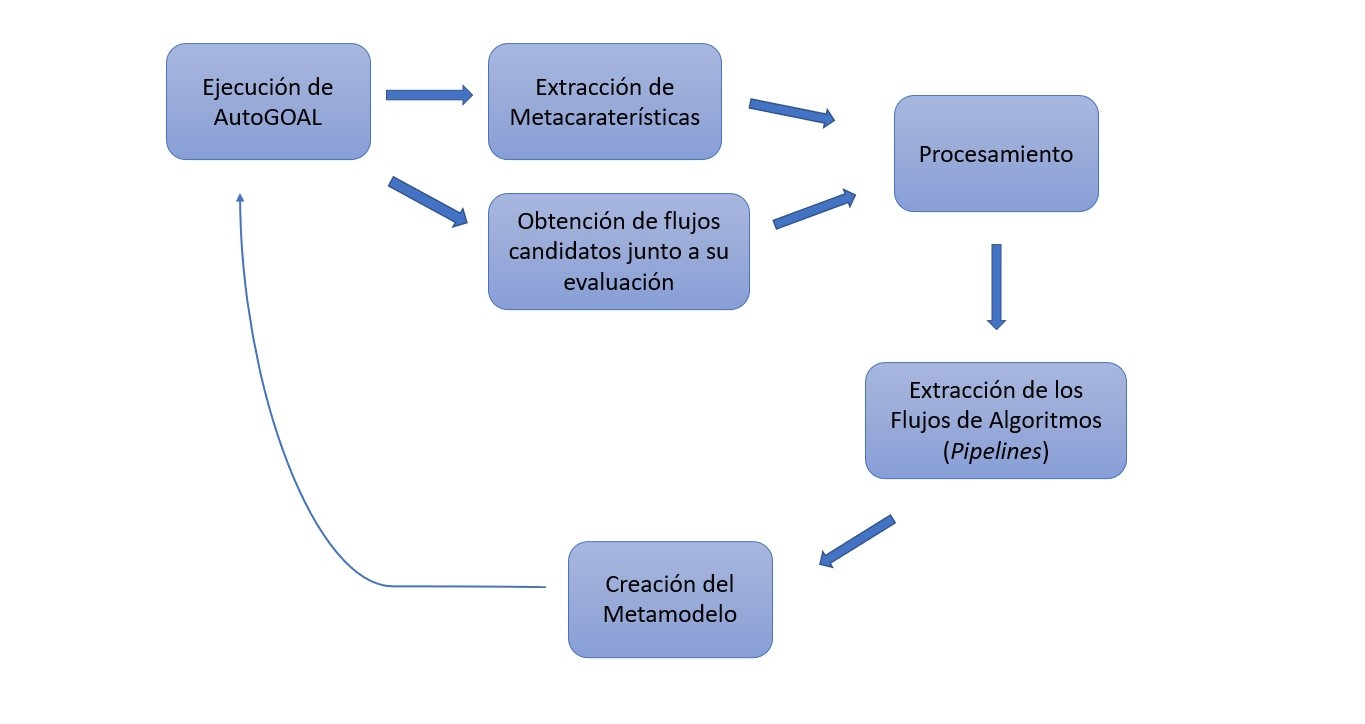
\includegraphics[scale=.5]{Figures/proposal-flow.jpg}
    \caption{Esquema del flujo la propuesta}
    \label{fig:prop-flow}
\end{figure}

Primeramente se realiza una ejecución de AutoGOAL~(sistema de AutoML usado en el
trabajo), con lo cual el sistema va a entrenarse en varios conjuntos de datos.
Luego se extraen características distintivas de estos problemas y se
seleccionan los flujos de algoritmos mejor ajustados al problema, medidos por
el resultado de efectividad que ofrecen. Posteriormente se procesan todos estos
datos los cuales servirán para un metamodelo. Dicho metamodelo servirá como
preentrenamiento de AutoGOAL y así en futuras ejecuciones dar buenos
resultados en un tiempo menor de ejecución.

%Explicar cad parte de la Propuesta

%Que se salva

\subsection{Ejecución de AutoGOAL}

Se realizan ejecuciones del sistema de AutoML producto de la necesidad de
usuarios de resolver problemas en los cuales se hace necesario esta herramienta.
Dichas ejecuciones sirven como datos para el análisis propuesto, donde se trata
de resolver problemas de manera más eficiente dada su similitud con algunos ya
analizados. 

\subsection{Análisis de los Conjuntos de Datos}

En la propuesta se tomaron varios conjuntos de datos, de los cuales se van a
extraer los características que los describen~(metacaracterísticas). Estas, como
ya se sabe, servirán para relacionar conjuntos de problemas, destacando
similitud para problemas futuros. De esta forma las soluciones a nuevos
problemas estarán relacionadas a las soluciones más factibles a problemas de
características similares. 

\subsection{Análisis de los Flujos de Algoritmos}

Producto de los análisis a los conjunto de datos, el modelo de entrenamiento
explora varios posibles flujo de algoritmos. Estos constituyen parte de los
datos de la exploración del modelo, junto con valor de efectividad el cual
cuantifica la calidad de un flujo dado contra dicho problema. Con estos datos
se filtran todas las posibles soluciones, buscando los flujos más factibles,
los cuales serán los más prometedores a problemas similares 

%Que procesamiento se hace

\section{Procesamiento}

El procesamiento es la fase principal de esta propuesta, es donde se analizan
los resultados de previas ejecuciones del sistema y se genera un modelo
preentrenado con mejores flujos de algoritmos para enfrentarse a nuevos
problemas.

\subsection{Selección de Flujos}

La selección de los flujos de algoritmos se hace bajo la premisa del análisis
de su valor de efectividad. Bajo esta premisa se garantiza que el nuevo modelo
se entrene con las mejores soluciones. De esta forma llegará más rápido a una
solución prometedora que resuelva el problema en cuestión sin la necesidad de
explorar un conjunto de soluciones a priori que solo sirvan para ralentizar la
ejecución del algoritmo. Dadas las características del proceso de optimización
con el cual el sistema de AutoML trabaja, con esta selección de flujos se
quiere reducir el espacio de búsqueda en función de reducir el tiempo de
espera. Por lo tanto se garantiza que se halla una solución con buen valor de
efectividad en un menor tiempo de ejecución.

\subsection{Creación del Metamodelo}

Con lo explicado anteriormente se crea el metamodelo que preentrena al sistema
de AutoML. El mismo se crea mediante un proceso de entrenamiento a partir de
problemas ya ejecutados en el sistema de AutoML, con los cuales buscará una
similitud a la hora de enfrentarse a otros nuevos, moviendo las soluciones en
un nuevo espacio de búsqueda más reducido que al hacerlo sin metalearning.

%que se obtiene

\section{Modelo con Metalearning}

Como resultado final se obtiene una herramienta más robusta de AutoML. El
concepto de metalearning busca brindarle a AutoGOAL una modificación de su
algoritmo de optimización el cual se basa en un modelo probabilístico. Esta
variación no busca un cambio en la cual AutoGOAL encuentra soluciones, sino
acotar el espacio de búsqueda probabilístico.
